\documentclass{article}
\usepackage[utf8]{inputenc}
\usepackage{geometry}
\usepackage{fancyhdr}
\usepackage{enumitem}
\usepackage{amsmath}
\usepackage{amssymb}
\usepackage{xcolor}
\usepackage{xfrac}
\usepackage{parskip}
\usepackage{tikz}
\setcounter{MaxMatrixCols}{20}

\geometry{margin=1in}
\pagestyle{fancy}
\fancyhf{}
\rhead{210 Notes}
\lhead{Class: Math 210, Sacramento State}
\cfoot{\thepage}

\title{Abstract Algebra Notes}
\author{Ryan Harris}
\date{\today}

\begin{document}

\maketitle

\setcounter{section}{-1}
\section{Introduction}
This document is a compilation of all notes taken in Dr. Craig Timmons' graduate level Abstract Algebra Class at California State University, Sacramento. Many of the sections follow those of Dummit and Foote's Abstract Algebra, 3rd Edition, though the notes are not directly aligned with the book. Specifically, many sections are ommitted, and many definitions, theorems, and examples are not from the book and do not follow a numbering system that is consistent with the book. Still, these notes may be very useful to students who are taking graduate level Abstract Algebra coursework.

For my comprehensive exams. Good luck G.

\section{Chapter 1: Introduction to Groups}
\subsection{Basic Axioms and Examples}

\textcolor{purple}{Definition 1.1.1:} A \textcolor{purple}{group} is a nonempty set $G$ with a binary operation $*$ from $G \times G \longrightarrow G$, where $G \times G = \{(g,h): g \in G, h \in H\}$. We may represent $*$ using notation that's more algebraic. For instance, we may write $g \times h$ or $gh$ instead of $f(g,h)$.

\textcolor{blue}{Example 1.1.1:} A binary operation on $S = \{1,2,3\}$ could be 
\[
\begin{array}{c|ccc}
    * & 1 & 2 & 3 \\ \hline
    1 & 1 & 1 & 1 \\
    2 & 1 & 1 & 1 \\
    3 & 1 & 1 & 1 \\
\end{array}
\]

A set $G$ with a binary operation $*$ is a \textcolor{purple}{group} if
\begin{enumerate}
    \item $a * (b * c) = (a * b) * c \ \forall a,b,c \in G$
    \item $\exists e \in G \text{ such that } a * e = a = e * a$
    \item for each $ a \in G$, $\exists b \in G$ such that $a * b = e = b * a$.
\end{enumerate}

That is, $G$ is a \textcolor{purple}{group} if $G$ is associative, contains an identity, and contains inverses for each element of $G$. We say $G$ is \textcolor{purple}{abelian} if $a * b = b * a \ \forall a,b \in G$ ($G$ is commutative). We say $G$ is a \textcolor{purple}{finite group} if $G$ as a set is finite (otherwise, $G$ is \textcolor{purple}{infinite}).

\textcolor{blue}{Example 1.1.2:} Some examples of groups include:
\begin{enumerate}
    \item $( \mathbb{Z}, +)$: integers under addition,
    \item $(\mathbb{Q}, +)$: rationals under addition,
    \item $(\mathbb{R}, +)$: reals under addition,
    \item $(\mathbb{C}, +)$: complex under addition,
    \item $(\mathbb{M}_{2 \times 2}\mathbb{R}, +)$: real $2$ by $2$ matrices under addition,
    \item $(\mathbb{Z}, \cdot)$: integers under multiplication,
    \item $(\mathbb{Q}\{0\}, \cdot)$: rationals (not including $0$) under multiplication,
    \item $(\mathbb{R}\{0\}, \cdot)=\mathbb{R}^*$: reals (not including $0$) under multiplication, and 
    \item for $n \in \mathbb{Z}^+$, $\mathbb{Z} / n\mathbb{Z} = \{\text{equivalence classes under the relation }a \sim b \longleftrightarrow n|(a-b),a,b \in \mathbb{Z}\}$.
\end{enumerate}

\textcolor{purple}{Definition 1.1.2:} The \textcolor{purple}{equivalence class} containing $a$ is denoted $\overline{a}$. We have $a = \{a+nk: k \in \mathbb{Z}\}$. Note that the operation is $\overline{a}+\overline{b}=\overline{a+b}$, where $\overline{a}+\overline{b}$ is addition under the group operation while $\overline{a+b}$ is the equivalence class containing $a+b$ where $a+b$ is the usual addition of integers.

\textcolor{blue}{Example 1.1.3:} \[
\begin{array}{c|cccc}
    \mathbb{Z}_4 & 0 & 1 & 2 & 3 \\ \hline
    0 & 0 & 1 & 2 & 3 \\
    1 & 1 & 2 & 3 & 0 \\
    2 & 2 & 3 & 0 & 1 \\
    3 & 3 & 0 & 1 & 2 \\
\end{array}
\]

The example above is the \textcolor{purple}{group of integers modulo n}. Note that in this case, $n=4$. For $n \in \mathbb{Z}^+,$ \\ $ \bigl( \sfrac{\mathbb{Z}}{n\mathbb{Z}} \bigr)^* = \{ \overline{a} \in \sfrac{\mathbb{Z}}{n\mathbb{Z}}: \gcd{(a,n)} = 1 \}$ and the operation is $\overline{a} \cdot \overline{b} = \overline{a \cdot b}$.\\

\textcolor{blue}{Example 1.1.4:} Some examples of modular groups include
\begin{enumerate}
    \item $\mathbb{Z}^*= (\{-1,1\}, \cdot$),
    \item $\mathbb{Z}_2 = (\{\overline{1}\}, \cdot$),
    \item $\mathbb{Z}_3 = (\{\overline{1}, \overline{2}\}, \cdot$),
    \item $\mathbb{Z}_4 = (\{\overline{1}, \overline{3}\}, \cdot$), and
    \item $GL_2(\mathbb{R}) = M_{2 \times 2}(\mathbb{R})^*$.
\end{enumerate}
Note that $GL_2(\mathbb{R})$ is the group of all invertible $2 \times 2$ matrices with real enteries under matrix multiplication and $M_{2 \times 2}(\mathbb{R})^*$ is the group of all $2 \times 2$ matrices with real entries under addition.

\textcolor{purple}{Definition 1.1.3:} A \textcolor{purple}{direct product} of two groups $(A,*)$ and $(B, \circ)$ is the group whose elements are $(a,b)$ where $a \in A, \ b \in B$, and the operation is $(a,b)(c,d) = (a * c, b \circ d)$.

\textcolor{orange}{Proposition 1.1.1:} If $(G, \cdot)$ is a group, then
\begin{enumerate}
    \item $e$ is unique in $G$,
    \item for each $a \in G$, $a^{-1}$ is unique,
    \item $(a^{-1})^{-1}=a$ $\forall a \in G$,
    \item $(ab)^{-1} = b^{-1}a^{-1} \ \forall a,b \in G$, and 
    \item for any $a_1, a_2, \dots, a_n \in G$, their product $a_1 \cdot a_2 \cdots a_n$ does not depend on how the expression is bracketed.
\end{enumerate}

Now, some comments on notation in groups. First, note that the default setting for group operations is multiplicative. That is, if $G$ is any group with $x \in G$, then
\begin{align*}
    x^0 &= e, \\
    x^n &= x \cdots x \ n \text{ times, } n \in \mathbb{Z}^+, \text{ and }\\
    x^{-n} &= x^{-1} \cdot x^{-1} \cdots x^{-1} \ n \text{ times, } n \in \mathbb{Z}^+ \\
    &= (x \cdot x \cdots x)^{-1} \text{ with } n \text{ many } x \text{'s}. 
\end{align*}

Next, note that if $G$ is abelian, we may change to additive notation. That is,
\begin{align*}
    a^{-1} &= -a, \\
    ab &= a+b, \\
    a^n &= a+a+ \cdots +a \ n \text{ times, } n \in \mathbb{Z}^+, \\
    e &=0, \text{ and } \\
    a^{-n}&= -na \\
    &= n(-a) \\
    &= (-a) + (-a) + \cdots + (-a) \ n \text{ times, } n \in \mathbb{Z}^+.
\end{align*}

\textcolor{purple}{Definition 1.1.4:} Let $D$ be a nonempty set. The \textcolor{purple}{power set} of $D$, $\mathcal{P}(D)$, is the set of all possible subsets of $D$. 

\textcolor{blue}{Example 1.1.5:} Let $D= \{a,b,c\}$. Then
\[
    \mathcal{P}(D) = \{ \emptyset, \{a\}, \{b\}, \{c\}, \{a,b\}, \{a,c\}, \{b,c\}, D \}.
\]

\textcolor{blue}{Example 1.1.6:} Define $A+B = (A \backslash B) \cup (B \backslash A)$ as an additive operation. Then 
\begin{align*}
    A+\emptyset &= (A \backslash \emptyset) \cup (\emptyset \backslash A), \\
    A^{-1} &= A \\
    &\Longrightarrow A+A = 2A = \emptyset.
\end{align*}

Then it turns out that $(\mathcal{P}(D),+)$ is an abelian group with $e^+ = \emptyset$. Observe that for any $A \in \mathcal{P}(D)$,
\begin{align*}
    A+A &= (A \backslash A) \cup (A \backslash A) \\
    &= \emptyset \\
    &= 2A.
\end{align*}
Note that every element then has order $2$ or $1$ (we will discuss order in the near future).

\textcolor{blue}{Example 1.1.7:} Let $G$ be a finite group. The operation table for $G = \{g_1, g_2, \dots, g_n\}$ is
\[
\begin{array}{c|cccccc}
    \cdot & g_1 & g_2 & \cdots & g_j & \cdots & g_n \\ \hline
    g_1 & g_1 \cdot g_1 & g_1 \cdot g_2 & \cdots & g_1 \cdot g_j & \cdots & g_1 \cdot g_n \\
    g_2 & g_2 \cdot g_1 & g_2 \cdot g_2 & \cdots & g_2 \cdot g_j & \cdots & g_2 \cdot g_n \\
    \vdots & \vdots & \vdots & \ddots & \cdots & \cdots & \vdots \\
    g_i & g_i \cdot g_1 & g_i \cdot g_2 & \cdots & g_i \cdot g_j & \cdots & g_i \cdot g_n \\
    \vdots & \vdots & \vdots & \ddots & \cdots & \cdots & \vdots \\
    g_n & g_i \cdot g_1 & g_n \cdot g_2 & \cdots & g_n \cdot g_j & \cdots & g_n \cdot g_n \\
\end{array}
\]

\textcolor{purple}{Definition 1.1.5:} If $G$ is a group with $x \in G$, then the \textcolor{purple}{order} of $x$, denoted $|x|$, is the smallest positive integer $n$ such that $x^n = e$. If no such $n$ exists, then $x$ has infinite order.

\textcolor{blue}{Example 1.1.8:} Let $\mathbb{C}^*$ be the group of nonzero complex numbers under multiplication. This group has elements of infinite order, such as $2$ or $2 + i$. There is also an element of order $1$ --- namely $e^*$. There is also an element of order $2$ (-1), and an element of order $4$ ($i$).

\subsection{Dihedral Groups and Group Actions}

\textcolor{purple}{Definition 1.2.1:} Let $G$ be a group and $A$ a set. A \textcolor{purple}{group action} of $G$ on $A$ is a function from $G \times A \longrightarrow A$ denoted $g \cdot a$ that satisfies
\begin{enumerate}
    \item $g_1 \cdot (g_2 \cdot a) = (g_1g_2) \cdot a \ \forall g_1, g_2 \in G$ and $\forall a \in A$ and 
    \item $e \cdot a = a \ \forall a \in A$.
\end{enumerate}
Note that for the items above, $\cdot$ denotes the group action, while the absence of $\cdot$ denotes the group operation on $G$. Further, $e$ is the identity in $G$.

\textcolor{blue}{Example 1.2.1:} Take $\mathbb{R}^*$ and $\mathbb{R}^n = \{(x_1, x_2, \dots, x_n)\: x_i \in \mathbb{R}\}$. Then
\[\alpha(x_1, x_2, \dots, x_n) = (\alpha x_1, \alpha x_2, \dots, \alpha x_n)\]
is a group action in which the group operation is scalar multiplication.

\textcolor{purple}{Definition 1.2.2:} For $n \geq 3$, the \textcolor{purple}{Dihedral Group} of order $2n$, denoted $D_{2n}$, is the set of symmetries of a regular $n$-gon.

\textcolor{blue}{Example 1.2.2:} $D_6 = D_{2 \cdot 3}$ is the set of symmetries of a regular $3$-gon (that is, of an equilateral triangle). The $6$ symmetries are
\begin{enumerate}
    \item rotate clockwise by $120^{\circ}$,
    \item rotate clockwise by $240^{\circ}$,
    \item reflect about vertical line of symmetry,
    \item reflect about left corner,
    \item reflect about right corner, and 
    \item keep it stationary.
\end{enumerate}
Let $r$ correspond to $120^{\circ}$ rotation and let $s$ correspond to the verticle reflection. Then we have \\
$D_6 = \{r, r^2, e, s, sr, sr^2\}$. Think of $r$ and $s$ as functions. That is, 

\begin{center}
    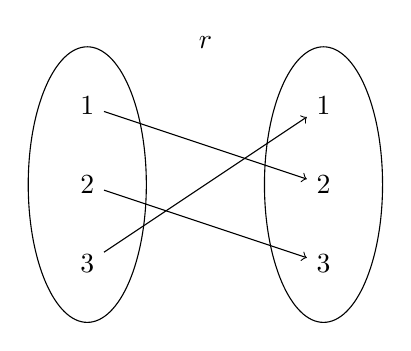
\begin{tikzpicture}
        \node (a1) at (0,2) {$1$};
        \node (a2) at (0,1) {$2$};
        \node (a3) at (0,0) {$3$};

        \node (b1) at (3,2) {$1$};
        \node (b2) at (3,1) {$2$};
        \node (b3) at (3,0) {$3$};

        \draw (0,1) ellipse (0.75cm and 1.75cm);
        \draw (3,1) ellipse (0.75cm and 1.75cm);

        \node at (1.5,2.8) {$r$};

        \draw[->] (a1) -- (b2);
        \draw[->] (a2) -- (b3);
        \draw[->] (a3) -- (b1);
    \end{tikzpicture}
\end{center}

Thus, we treat the dihedral group of order $6$ (or of any other order) like function composition. That is, $sr = s \circ r$, so 

\begin{center}
    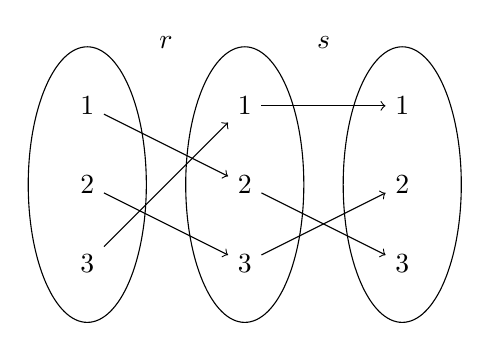
\begin{tikzpicture}
        \node (a1) at (0,2) {$1$};
        \node (a2) at (0,1) {$2$};
        \node (a3) at (0,0) {$3$};

        \node (b1) at (2,2) {$1$};
        \node (b2) at (2,1) {$2$};
        \node (b3) at (2,0) {$3$};

        \node (c1) at (4,2) {$1$};
        \node (c2) at (4,1) {$2$};
        \node (c3) at (4,0) {$3$};

        \draw (0,1) ellipse (0.75cm and 1.75cm);
        \draw (2,1) ellipse (0.75cm and 1.75cm);
        \draw (4,1) ellipse (0.75cm and 1.75cm);

        \node at (1,2.8) {$r$};
        \node at (3, 2.8) {$s$};

        \draw[->] (a1) -- (b2);
        \draw[->] (a2) -- (b3);
        \draw[->] (a3) -- (b1);
        \draw[->] (b1) -- (c1);
        \draw[->] (b2) -- (c3);
        \draw[->] (b3) -- (c2);
    \end{tikzpicture}
\end{center}

The notation we will use with $D_{2n}$ is $D_{2n} = \{e,r,r^2, \dots, r^{n-1},s,sr, \dots, sr^{n-1}\}$.

\textcolor{purple}{Definition 1.2.3:} Let $G$ be a group acting on a set $A$ with $a \in A$. The \textcolor{purple}{stabilizer} is the set $Stab(a) = \{g \in G: g \cdot a = a\}$. Next, we prove that the stabilizer forms a subgroup.

\textbf{Proof:} Let $G$ and $A$ be defined as above with $a \in A$. Since $G$ is a group, $e \in G$. Further, $e \cdot a = a$, so $e \in Stab(a)$, and thusly $Stab(a) \neq \emptyset$. 

Next, let $g,h \in Stab(a)$. Then $g \cdot a = a$ and $h \cdot a = a$. We want to show $(gh) \cdot a = a$. By definition of a group action, we know
\begin{align*}
    (gh) \cdot a &= g \cdot (h \cdot a) \\
    &= g \cdot a \\
    &= a
\end{align*}
Then $(gh) \cdot a = a$, so $(gh) \in Stab(a)$. Next, we need to show $g^{-1} \in Stab(a)$. Consider $g \cdot a = a$. Then we have
\begin{align*}
    g^{-1} \cdot a &=  g^{-1} \cdot (g \cdot a)\\
    &= (g^{-1}g) \cdot a \\
    &=e \cdot a \\
    &= a
\end{align*}
Then, since $a \in Stab(a)$, we must have that $g^{-1} \in Stab(a) \ \forall g \in Stab(a)$. Then $Stab(a) \leq G$. $\square$

\textcolor{blue}{Example 1.2.4:} Let $G$ act on $G$ by the rule $g \cdot x = gxg^{-1}$. Let's check that this defines an action. For any $x \in G$, $e \cdot x = e \cdot x \cdot e^{-1} = x$. Next, for any $g,h \in G$ and $x \in G$, we have
\begin{align*}
    (g \cdot h) \cdot x &= g \cdot (h \cdot x)  \\
    &= g \cdot (hxh^{-1}) \\
    &= g(hxh^{-1})g^{-1} \\
    &= (gh)x(h^{-1}g^{-1}) \\
    &= (gh)x(gh)^{-1} \\
    &= (gh)x 
\end{align*}
so we must have that $g \cdot x = gxg^{-1}$ defines an action of $G$ on $G$. Next, what is $Stab(x)$?
\begin{align*}
    Stab(x) &= \{ g \in G: g \cdot x = x\} \\
    &= \{ g \in G: gxg^{-1} = x\} \\
    &= \{ g \in G: gx = xg\} \\
    &= C(x) \text{ or } C_G(x)
\end{align*}
\textcolor{purple}{Definition 1.2.4:} Let $G$ be a group with $g \in G$ and $x \in A$ with $A$ a set. The collection of elements in $G$ that commute with $x$ is called the \textcolor{purple}{centralizer} of $x$ and is denoted $C(x)$ or $C_G(x)$. Similarly, if $S$ is a set, then $C(S) = \{ g \in G: gx = xg \ \forall x \in S\}$. Note that this is not to be confused with the \textcolor{purple}{center} of $G$, defined below.

\textcolor{purple}{Definition 1.2.5:} Let $G$ be a group. Then the \textcolor{purple}{center} of $G$ is $Z(G) = \{g \in G: gx = xg \ \forall x \in G\}$. That is, the center of $G$ is the set of all elements in $G$ which commute with every element of $G$. Note that $Z(G) = G \Longrightarrow G$ is abelian.

Now, some notes on notation and a relation that is used in $D_{2n}$. Remember, $D_{2n} = \{e,r,r^2, \dots, r^{n-1}, s, sr, sr^2, \dots, sr^{n-1}\}$. Then $|r| = n$ and $|s|=2$, where $r$ denotes a rotation and $s$ denotes a reflection. Further, $r^is = sr^{-i}$ $\forall 0 \leq i \leq n$. In particular, when $i=1$, $rs = sr^{-1} = sr^{n-1}$. Similarly, $r^{n-1}s = sr$.

\textcolor{blue}{Example 1.2.5:} Let $n=5$. Then $r^3s = sr^{-3} = sr^2$ with $D_{2 \cdot 5} = \{e,r,r^2,r^3,r^4,s,sr,sr^2,sr^3,sr^4\}$. Next, let $n=15$. Then $rsr^3 = rr^{12}s = r^{13}s$. Lastly, let $n = 12$. Then 
\begin{align*}
    (sr^9)(sr^6) &= sr^9r^{-6}s \\
    &= sr^3s \\
    &= r^{-3}ss \\
    &= r^9e \\
    &= r^9.
\end{align*}

\subsection{Symmetric Groups}
\textcolor{purple}{Definition 1.3.1:} Let $\Omega$ be a nonempty set. Let $S_{\Omega}$ be the set of all bijections from $\Omega$ to $\Omega$. The set $S_{\Omega}$ forms a group, the \textcolor{purple}{symmetric group on $\Omega$}, under function composition. The identity function in this set is denoted $\mathbb{1}$, or sometimes $Id(S_{\Omega})$. What this means is $\mathbb{1}(x)=x$ $\forall x \in \Omega$.

In a special case that this set $\Omega = \{1,2,3, \dots, n\}$, we write $S_n$ instead of $S_{1,2,3,\dots,n}$. $S_n$ is called the \textcolor{purple}{symmetric group of degree $n$}. Elements in $S_n$ are called \textcolor{purple}{permutations}.

\textcolor{blue}{Example 1.3.1:} One way we can represent permutations is with two line notation, as seen below:

Let $\alpha \in S_7$ such that $\alpha(1)=5, \alpha(2) = 1, \alpha(3)=7, \alpha(4)=6, \alpha(5)=2, \alpha(6)=4,$ and $\alpha(7)=3$. Then the two line notation for $\alpha$ looks like 

\[
    \alpha = \begin{pmatrix}
        1 & 2 & 3 & 4 & 5 & 6 & 7 \\
        5 & 1 & 7 & 6 & 2 & 4 & 3
    \end{pmatrix}.
\]

\textcolor{blue}{Example 1.3.2:} In $S_6$, if $\beta = \begin{pmatrix}
    1 & 2 & 3 & 4 & 5 & 6 \\
    1 & 5 & 2 & 4 & 3 & 6
\end{pmatrix}$, then $\beta = (2 \ 5 \ 3)$. 

\textcolor{purple}{Definition 1.3.2:} Two cycles $(a_1 \ a_2 \ \cdots \ a_n)$ and $(b_1 \ b_2 \ \cdots b_m)$ are \textcolor{purple}{disjoint} if $\{a_1, a_2, \dots, a_n\} \cap \{b_1, b_2, \dots, b_m\} = \emptyset$. 

\textcolor{blue}{Example 1.3.3:} In $S_7$, $\alpha = \begin{pmatrix}
    1 & 2 & 3 & 4 & 5 & 6 & 7 \\
    5 & 1 & 7 & 6 & 2 & 4 & 3
\end{pmatrix} = (1 \ 5 \ 2)(3 \ 7)(4 \ 6) \text{ and in } S_{13}$,
\begin{align*}
\theta &= \begin{pmatrix}
        1 & 2 & 3 & 4 & 5 & 6 & 7 & 8 & 9 & 10 & 11 & 12 & 13 \\
        12 & 13 & 3 & 1 & 11 & 9 & 5 & 10 & 6 & 4 & 7 & 8 & 2
    \end{pmatrix} \\
    &= (1 \ 12 \ 8 \ 10 \ 4)(2 \ 13)(3)(5 \ 11 \ 7)(6 \ 9) \\
    &= (1 \ 12 \ 8 \ 10 \ 4)(2 \ 13)(5 \ 11 \ 7)(6 \ 9). 
\end{align*}

It is useful to note that $1$-cycles are typically ommitted from products of cycles. Further, it is important to note that disjoint cycles commute.

\textcolor{purple}{Definition 1.3.3:} The \textcolor{purple}{length} of cycle $(a_1 \ a_2 \ \cdots \ a_n)$ is $n$, and this is commonly referred to as an \textcolor{purple}{$n$-cycle}. Further, note that $2$-cycles are also called \textcolor{purple}{transpositions}.

\textcolor{blue}{Example 1.3.4:} Let us write all elements of $s_4$ as products of disjoint cycles. First, we start with the $1$-cycle --- 
namely, $\{(1)\}$. Note that we could have written this as $\{(2)\}, \ \{(3)\}$, or $\{(4)\}$. Next, we consider the 
$2$-cycles. We have 
\[
    \{(1 \ 2),(1 \ 3),(1 \ 4),(2 \ 3),(2 \ 4),(3 \ 4)\}.
\]
The set of $3$-cycles includes 
\[
    \{(1 \ 2 \ 3), (1 \ 3 \ 2), (1 \ 2 \ 4), (1 \ 4 \ 2), (1 \ 3 \ 4), (1 \ 4 \ 3), (2 \ 3 \ 4), (2 \ 4 \ 3)\}.
\]
Next, the set of $4$-cycles is 
\[
    \{(1 \ 2 \ 3 \ 4), (1 \ 2 \ 4 \ 3), (1 \ 3 \ 2 \ 4), (1 \ 3 \ 4 \ 2), (1 \ 4 \ 2 \ 3), (1 \ 4 \ 3 \ 2)\}.
\]
The last cycle-type present in $S_4$ is the $2$-$2$-cycle, of which there are three: $\{(1 \ 2)(3 \ 4), (1 \ 3)(2 \ 4), (1 \ 4)(2 \ 3)\}$.
Note that there is one $1$-cycle and there are six $2$-cycles, eight $3$-cycles, and six $4$-cycles. This brings us to 
an interesting question --- how many permutations in $S_n$ have a given cycle type?

\textcolor{blue}{Example 1.3.5:} How many permutations have each cycle type in $S_5$?
\[
    \begin{array}{c|c|c}
        \text{Cycle Type} & \text{Number of permutations with given cycle type} & \text{example} \\
        \hline \\
        1\text{-cycle} & 1 & (1) \\
        2\text{-cycle} & \dfrac{5 \cdot 4}{2} = 10 & (1 \ 2) \\[6pt]
        3\text{-cycle} & \dfrac{5 \cdot 4 \cdot 3}{3}= 20 & (1 \ 2 \ 3) \\[6pt]
        4\text{-cycle} & \dfrac{5 \cdot 4 \cdot 3 \cdot 2}{4}=30 & (1 \ 2 \ 3 \ 4) \\[6pt]
        5\text{-cycle} & \dfrac{5 \cdot 4 \cdot 3 \cdot 2 \cdot 1}{5}=24 & (1 \ 2 \ 3 \ 4 \ 5) \\[6pt]
        3\text{-}2\text{-cycle} & \dfrac{5 \cdot 4 \cdot 3}{3} \cdot \dfrac{2 \cdot 1}{2} = 20 & (1 \ 2 \ 3)(4 \ 5) \\[6pt]
        2\text{-}2\text{-cycle} & \dfrac{\dfrac{5 \cdot 4}{2} \cdot \dfrac{3 \cdot 2}{2}}{2} = 15 & (1 \ 2)(3 \ 4)
    \end{array}
\]
Note that the total number of permutations in $S_n$ is $n!$.

\textcolor{blue}{Example 1.3.6:} Consider $S_{50}$. How many $2$-$3$-$3$-cycles are there?
\[
    \dfrac{50 \cdot 49}{2} \cdot \dfrac{\dfrac{48 \cdot 47 \cdot 46}{3} \cdot \dfrac{45 \cdot 44 \cdot 43}{3}}{2}=601,304,088,000.
\]

\textcolor{purple}{Definition 1.3.3:} Let $G$ be a group. For $x,y \in G$, lets say that $x$ is a \textcolor{purple}{conjugate} of $y$ if $x = gyg^{-1}$ for some
$g \in G$. Another notation for this is to say that $x \in cl(y)$, or $x \sim y$. Further, the \textcolor{purple}{conjugacy class} that contains $y$ is
$cl(y) = \{gyg^{-1}:g \in G\}$. 

\textcolor{blue}{Example 1.3.7:} In $S_3$, what is $cl((1 \ 2))$? To find out, we must find all unique conjugates of $(1 \ 2)$. We have
\begin{align*}
    (1)(1 \ 2)(1)^{-1} &= (1 \ 2) \\
    (1 \ 2)(1 \ 2)(1 \ 2)^{-1} &= (1 \ 2) \\
    (1 \ 3)(1 \ 2)(1 \ 3)^{-1} &= (1 \ 3)(1 \ 2)(3 \ 1) = (1)(2 \ 3) = (2 \ 3) \\
    (2 \ 3)(1 \ 2)(2 \ 3)^{-1} &= (2 \ 3)(1 \ 2)(3 \ 2) = (1 \ 3)(2) = (1 \ 3) \\
    (1 \ 2 \ 3)(1 \ 2)(1 \ 2 \ 3)^{-1} &= (1 \ 2 \ 3)(1 \ 2)(3 \ 2 \ 1) = (1)(2 \ 3) = (2 \ 3) \\
    (1 \ 3 \ 2)(1 \ 2)(1 \ 3 \ 2)^{-1} &= (1 \ 3 \ 2)(1 \ 2)(2 \ 3 \ 1)^{-1} = (1 \ 3)(2) = (1 \ 3).
\end{align*}
Then $cl((1 \ 2)) = \{(1 \ 2), (1 \ 3), (2 \ 3)\}$.

\textcolor{red}{Theorem 1.3.1:} The relation $\sim$ is an equivalence relation on $G$.

\textbf{Proof:} First, we will show that $\sim$ is reflexive. Note that $x \sim x$ $\forall x \in G$ since $x = exe^{-1} \ \forall x \in G$. Next, we need to show that $\sim$ is symmetric. 
Suppose $x \sim y$. Then we have
\begin{align*}
    x \sim y &\Longrightarrow x = gyg^{-1} \text{ for some } g \in G \\
    &\Longrightarrow g^{-1}x = g^{-1}gyg^{-1} \\
    &\Longrightarrow g^{-1}x = yg^{-1} \\
    &\Longrightarrow g^{-1}xg = yg^{-1}g \\
    &\Longrightarrow g^{-1}xg = y \\
    &\Longrightarrow y = (g^{-1})x(g^{-1})^{-1} \\
    &\Longrightarrow y \sim x,
\end{align*}
so $\sim$ is symmetric. Lastly, we check for transitivity. Suppose $x \sim y$ and $y \sim z$. Then $x = gyg^{-1}$ and $y = hzh^{-1}$ for some $g,h \in G$. Then
\begin{align*}
    x &= g(hzh^{-1})g^{-1} \\
    &= (gh)z(h^{-1}g^{-1}) \\
    &= (gh)z(gh)^{-1} \\
    &\Longrightarrow x \sim z,
\end{align*}
so $\sim$ is transitive. Then $\sim$ is an equivalence relation on $G$. $\square$

One last observation that is important to note is that $x \in cl(x)$. Next, we claim that $|cl(x)| = 1$ if and only if $x \in Z(G)$. 

\textbf{Proof:} Assume the order of the closure of $x$ is one. Then we have
\begin{align*}
    |cl(x)|=1 &\Longleftrightarrow \{x\} = cl(x) \\
    &\Longleftrightarrow \{x\} = \{gxg^{-1}:g \in G\} \\
    &\Longleftrightarrow x = gxg^{-1} \ \forall g \in G \\
    &\Longleftrightarrow xg = gxg^{-1}g \ \forall g \in G \\
    &\Longleftrightarrow xg = gx \ \forall g \in G \\
    &\Longleftrightarrow x \in Z(G). \ \square 
\end{align*}
Our big takeaway from this is that conjugacy classes partition the group. Further, if $\{x\}$ is a conjugacy class, then $x \in Z(G)$. In particular, when $G$ is a finite group, it's order can be described as follows:
\[
    |G| = |Z(G)| + \sum{|cl(x)|}
\]
where the summation is taken over the distinct conjugacy classes of size more than one. The equation above is known as the \textcolor{purple}{Class Equation}, which we will discuss soon. Note that we can write the class equation in terms of centralizers (subgroups of the form $C_G(x)$).

\textcolor{blue}{Example 1.3.8:} Consider $S_4$. Then we have 
\begin{align*}
    |S_4| &= 1+|cl((1 \ 2))|+|cl((1 \ 2 \ 3))|+|cl((1 \ 2 \ 3 \ 4))|+|cl((1 \ 2)(3 \ 4))| \\
    24 &= 1 + 6 + 8 + 6 + 3
\end{align*}
Note that for each conjugacy class, it divides the order of the group. That is, $|cl(x)| \big| |G|$. 

It is important to note some important facts on the order of groups before we move on. First, if $G$ is a group of even order, then $G$ has an element of order $2$. Further, if the order of a group $G$ is the power of a prime (that is, if $|G| = p^n$ with $p$ prime), then $Z(G) \neq 1$.

\textcolor{purple}{Definition 1.3.4:} Let $G$ be a group with $H \subseteq G$. For $x \in G$, define $xH = \{xh: h \in H\}$ and $Hx = \{hx: h \in H\}$. When $H \leq G$, we call $xH$ a \textcolor{purple}{left coset} of $H$ in $G$ and $Hx$ a \textcolor{purple}{right coset} of $H$ in $G$. 

Recall that $G_G(x) \{y \in G: yx=xy\}$. Can we say anything if $aC_G(x) = bC_G(x)$? Consider the following claim:
Let $H \leq G$. Then $xH=yH$ if and only if $y^{-1}x \in H$.\\
\textbf{Proof:} Suppose $xH=yH$. Then $xh_1=yh_2$ for some $h_1,h_2 \in H$. We have
\begin{align*}
    xh_1 = yh_2 &\Longleftrightarrow x=yh_2h_1^{-1} \\
    &\Longleftrightarrow y^{-1}x = y^{-1}yh_2h_1^{-1} \\
    &\Longleftrightarrow y^{-1}x=h_2h_1^{-1}
\end{align*}
Note that, since $h_1,h_2 \in H$, we must have that $h_1^{-1} \in H$ and $h_2h_1^{-1}\in H$. Then $y^{-1}x\in H$. $\square$

Next, let $A$ be the set of all left cosets of $C_G(x)$ in $G$. That is, let $A = \{yC_G(x):y \in G\}$. Next, define a function $f: A \longrightarrow cl(x)$ by $f(yC_G(x)) = yxy^{-1}$. We claim that $f$ is a bijection.\\

\textbf{Proof:} Let $axa^{-1}\in cl(x)$. Then $f(aC_G(x)) = axa^{-1}$, so $\exists aC_G(x) \in A$, and thusly $f$ is onto.

Next, suppose you have two equal outputs $f(aC_G(x))=f(bC_G(x))$. Then we have $axa^{-1}=bxb^{-1}$. But this implies $aC_G(x)=bC_G(x)$, so we must have that $f$ is one-to-one. $\square$.

By an earlier claim, for any $x \in G$, the number of conjugates of $x$ is the same as the number of left cosets of $C_G(x)$ in $G$. Notationally speaking, for $H \leq G$, we write $[G:H]$ (which reads as the \textcolor{purple}{index} of $H$ in $G$), for the number of left cosets of $H$ in $G$. Then we would say $|cl(x)| = [G:H]$.

This brings our discussion on the order of groups to the Class equation --- but first, we must define another theorem.

\textcolor{red}{Theorem 1.3.2:} Let $G$ be a group, $x \in G$, and $C_G(x)$ be the centralizer of $x$ in $G$. Then \textcolor{red}{La Grange's Theorem} states that the index of $C_G(x)$ in $G$ is equal to the order of $G$ divided by the order of $C_G(x)$. That is,
\[
    [G:C_G(x)] = \dfrac{|G|}{|C_G(x)|}.
\]
We will use this to better understand the equation given below.

\textcolor{purple}{Definition 1.3.5:} Given a finite group $G$, the \textcolor{purple}{Class Equation} states that 
\[
    |G| = |Z(G)| + \sum{|cl(x)|}.
\]
That is, the number of elements in $G$ is equal to the number of commutative elements in $G$ plus the sum of the sizes of conjugacy classes containing $x$ where that sum is taken over all conjugacy classes of size more than one with just one $x$ per conjugacy class. Now, we can write this similarly with indeces:
\[
    |G| = |Z(G)|+\sum{[G:C_G(x)]},
\]
where the sum is taken in the same method as the previous version of the Class Equation.

This brings us to an interest result. We claim that if the order of a group $G$ is equal to the power of a prime $p$, then there exists some $x$ in the center of $G$ such that $x$ is not the identity element. This brings us to an important theorem.

\textcolor{red}{Theorem 1.3.3:} Let $p$ be a prime. If $G$ is a group with $|G = p^k$, $k \in \mathbb{Z}^+$, then $|Z(G)| \geq p$.\\
\textbf{Proof:} By the class equation, $|G| = |Z(G)| + \sum{[G:C_G(x)]}$, where the sum is taken over all conjugacy classes of size more than one with one $x$ per conjugacy class. Then, since $|G|= p^k$ and $[G:C_G(x)] = \dfrac{|G|}{|C_G(x)|}$ by La Grange, we must have
\[
    p^k = |Z(G)+\sum{\dfrac{p^k}{|C_G(x)|}}.
\]
Note that, since we are only taking the sum over all conjugacy classes of size mroe than one with one $x$ per conjugacy class, we must have that $|C_G(x)| <p^k$. In other words, if $|C_G(x)| = p^k$, then we must have that $x \in Z(G)$. But we don't want to count any of the $x$'s more than once.
Then $\forall x \notin Z(G)$, $C_G(x) \nleq G$. By La Grange, $|C_G(x)| \big| |G| = p^k$. Then $|C_G(x)| = p^{l_x}$ for some $0 \leq l_x < k$. This means that each term $\dfrac{p^k}{|C_G(x)|} = p^{k-l_x}$, which is divisible by $p$.
Then $\sum{\dfrac{p^k}{|C_G(x)|}}$ (where the sum is again taken over all conjugacy classes of size more than one with one $x$ per conjugacy class) is the sum of elements that are all divisible by $p$. Thus, the entire sum is divisible by $p$. Then we have
\[
    p^k = |Z(G)|+\sum{\dfrac{p^k}{|C_G(x)|}} \text{ and} 
\]
\[
    p^k-\sum{\dfrac{p^k}{|C_G(x)|}} \text{ divides } p.
\]
Thusly, $|Z(G)| \big| p$, so we must have that $|Z(G)| \geq p$ and $Z(G)$ contains a non-identity element. $\square$

\setcounter{subsection}{5}
\subsection{Homomorphisms and Isomorphisms}
\textcolor{purple}{Definition 1.6.1:} Let $(G, \cdot)$ and $(H, \circ)$ be groups. A function $\phi:G \longrightarrow H$ is a \textcolor{purple}{homomorphism} if
\[
    \phi(g_1 \cdot g_2) = \phi(g_1) \circ \phi(g_2) \ \forall g_1, g_2 \in G.
\]
Note that typically this is written in shorthand as $\phi(g_1g_2) = \phi(g_1)\phi(g_2)$. 

\textcolor{purple}{Definition 1.6.2:} A bijective homomorphism is called an \textcolor{purple}{isomorphism}. If there is an isomorphism from $G$ to $H$, we write $G \cong H$ and say $G$ is \textcolor{purple}{isomorphic} to $H$.

\textcolor{blue}{Example 1.6.1:} Let $(\mathbb{R},+)$ be the group of real numbers under addition and let $(\mathbb{R}^+, \cdot)$ be the group of positive real numbers under multiplication. Then the function $f:\mathbb{R} \longrightarrow \mathbb{R}^+$ defined by $f(x)=e^x$ is an isomorphism. \\
To show this, first, we must check that $f$ is a homomorphism. Let $x_1, x_2 \in \mathbb{R}$. Then
\begin{align*}
    f(x_1+x_2) &= e^{x_1+x_2} \\
    &= e^{x_1}e^{x_2} \\
    &= f(x_1)f(x_2).
\end{align*}
Then $f$ is operation preserving and thusly a homomorphism. To check that this is also an isomorphism, we must check that $f$ is a bijection. First, we check that $f$ is one-to-one. Let $f(x_1)=f(x_2)$. Then we have 
\begin{align*}
    f(x_1)=f(x_2) &\Longrightarrow e^{x_1} = e^{x_2} \\
    &\Longrightarrow \ln{e^{x_1}} = \ln{e^{x_2}} \\
    &\Longrightarrow x_1 = x_2,
\end{align*}
so $f$ is one-to-one. Next, we check that $f$ is onto. Let $y = f(x)$. Then $y = e^x$ and we have $\ln{y} = \ln{e^x}$, so $\ln{y}=x$. Thusly, we have
\[
    f(\ln{y}) = e^{\ln{y}} = y,
\]
so $f$ is onto. Then $f$ is a bijective homomorphism, and thusly, $f$ is an isomorphism. 

Interestingly, isomorphisms preserve may properties. Assume $\phi: G \longrightarrow H$ is a function with $G$ isomorphic to $H$. Then we have
\begin{enumerate}
    \item $|G| = |H|$ 
    \item $ord_G(x) = ord_H(x)$
    \item $G$ is abelian $\Longleftrightarrow H$ is abelian
    \item $G$ is cyclic $\Longleftrightarrow H$ is cyclic
\end{enumerate}

\textcolor{blue}{Example 1.6.2:} Is $(\mathbb{R}, +) \cong (\mathbb{R} \backslash \{0\}, \cdot)$?\\
No! Consider $(-1)^2 = e \in (\mathbb{R} \backslash \{0\}, \cdot)$. Then that $|-1| = 2$ but $\nexists x \in (\mathbb{R}, +)$ such that $|x|=2$ and $x \neq e$.

Now, let us look at a particular family of permutations coming from group actions:

Consider the group $G$ and set $A$ with a fixed $g \in G$. Let our group $G$ act on set $A$ via group action $G \times A \longrightarrow A$ be defined by 
\begin{center}
    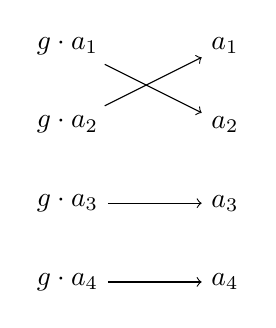
\begin{tikzpicture}
        \node (a1) at (0,3) {$g \cdot a_1$};
        \node (a2) at (0,2) {$g \cdot a_2$};
        \node (a3) at (0,1) {$g \cdot a_3$};
        \node (a4) at (0,0) {$g \cdot a_4$};
        
        \node (b1) at (2,3) {$a_1$};
        \node (b2) at (2,2) {$a_2$};
        \node (b3) at (2,1) {$a_3$};
        \node (b4) at (2,0) {$a_4$};

        \draw[->] (a1) -- (b2);
        \draw[->] (a2) -- (b1);
        \draw[->] (a3) -- (b3);
        \draw[->] (a4) -- (b4);
    \end{tikzpicture}
\end{center}

Then we can associage to $g$ a map $\sigma_g: A \longrightarrow A$ where $\sigma_g(a) = g \cdot a$. It turns out that $\sigma_g$ is a bijection, and thus it is a permutation on $A$.
\textbf{Proof:} Suppose $\sigma_g(a_1) = \sigma_g(a_2)$. Then we must have
\begin{align*}
    g \cdot a_1 = g \cdot a_2 &\Longrightarrow g^{-1} \cdot (g \cdot a_1) = g^{-1} \cdot(g \cdot a_2) \\
    &\Longrightarrow (g^{-1} g) \cdot a_1 = (g^{-1}g) \cdot a_2 \\
    &\Longrightarrow e \cdot a_1 = e \cdot a_2 \\
    &\Longrightarrow a_1 = a_2.
\end{align*}
Then $\sigma_g$ is one-to-one. Next, let $a \in A$. We want to find $\sigma_g(a)=a$. Consider $g^{-1} \cdot a \in A$. Then
\begin{align*}
    \sigma_g(g^{-1} \cdot a) &= g \cdot (g^{-1} \cdot a) \\
    &= (gg^{-1}) \cdot a \\
    &= e \cdot a \\
    &= a.
\end{align*}
Then $\sigma_g$ is a bijection and therefore a permutation on $A$. $\square$

Now, is this map operation preserving? In other words, is this map a homomorphism?

\textbf{Proof:} Remember, group $G$ acts on set $A$ with the action denoted by $g \cdot a$. For $g \in G$, we define a function
\[
    \sigma_g:A \longrightarrow A
\]
by the rule $\sigma_g(a)=g \cdot a$ for $a \in A$. We We proved that $\sigma_g$ is one-to-one and onto, so it is a permutation of $A$.
Define $\phi: G \longrightarrow S_A$ by the rule $\phi(g) = \sigma_g$. Now, let $g_1,g_2 \in G$. 

$\phi(g_1g_2) = \sigma_{g_1g_2}$. Now for any $a \in A$,
\begin{align*}
    \sigma_{g_1g_2}(a) &= (g_1g_2) \cdot a \\
    &= g_1 \cdot(g_2 \cdot a) \\
    &= \sigma_{g_1}(g_2 \cdot a) \\
    &= \sigma_{g_1}(\sigma_{g_2}(a)) \\
    &= \sigma_{g_1} \circ \sigma_{g_2}(a).
\end{align*}
This shows that $\sigma_{g_1g_2} = \sigma_{g_1} \circ \sigma_{g_2}$. therefore
\begin{align*}
    \phi(g_1 g_2) &= \sigma_{g_1g_2} \\
    &= \sigma_{g_1} \circ \sigma_{g_2} \\
    &= \phi(g_1) \circ \phi(g_2). \ \square
\end{align*}

\textcolor{purple}{Definition 1.6.3:} The map $\phi$ is called the \textcolor{purple}{permutation representation of the action}. If $\phi$ is one-to-one (this means distinct elements of $G$ give distinct permutations of $A$), then the action is said to be \textcolor{purple}{faithful}.

\textcolor{purple}{Definition 1.6.4:} The \textcolor{purple}{kernel} of $G$ acting on a set $A$ is $\{g \in G: g \cdot a = a \ \forall a \in A\}$. This is the same thing as $\ker{(\phi)} = \{g \in G: \phi(g) = id_A\}$, where $id_A$ is the identity element in $S_A$.

\textcolor{blue}{Example 1.6.3:} Look at the cosets of $H = <(1 \ 2)> = \{(1 \ 2),(1)\}$ in $G = S_3$. Let $A = \{(1),H, (1 \ 3)H, (2 \ 3)H\}$. Then $G$ acts on $A$ by the rule $\alpha \cdot \beta H = \alpha\beta H$, where $\alpha \in G$, $\beta H$ is a coset in $A$, and $\alpha \beta H$ is a coset in $A$.
\[
    \begin{tabular}{c|c|c}
        (1)H & (1 \ 3)H & (2 \ 3)H \\
        \hline 
        (1 \ 2) & (1 \ 2 \ 3) & (1 \ 3 \ 2) \\
        (1) & (1 \ 3) & (2 \ 3)
    \end{tabular}
\]
Lets try $\alpha = (1 \ 2)$. Then we have
\begin{align*}
    (1 \ 2)(1)H &= (1 \ 2)H = (1)H \\
    (1 \ 2)(1 \ 3)H &= \{(1 \ 2)(1 \ 2 \ 3),(1 \ 2)(1 \ 3)\} \\
    &= \{(2 \ 3),(1 \ 3 \ 2)\} = (2 \ 3)H.
\end{align*}

\newpage 
\section{Chapter 2: Subgroups}
\subsection{Subgroups and Examples}
\textcolor{purple}{Definition 2.1.1:} Let $G$ be a group. The subset $H$ of $G$ is a \textcolor{purple}{subgroup} of $G$ if $H$ is nonempty and $H$ is closed under products and inverses. That is, $H$ is a subgroup of $G$ if
\begin{enumerate}
    \item $xy \in H \ \forall x,y \in H$ and 
    \item $x^{-1} \in H \ \forall x \in H$.
\end{enumerate}
If $H$ is a subgroup of $G$ then we write $H \leq G$.

\textcolor{blue}{Example 2.1.1:} Consider the following examples of subgroups:
\begin{enumerate}
    \item $\mathbb{Z} \leq \mathbb{Q}$ and $\mathbb{Q} \leq \mathbb{R}$ (both under addition).
    \item Any group $G$ has at least two subgroups --- $H = G$ and $H = \{e\}$. Note that the latter is called the \textcolor{purple}{trivial subgroup} (this is denoted by $1$ in Dummit and Foote).
    \item Let $G = D_{2n}$ be the dihedral group of order $2n$, and let $H = \{1,r,r^2, \dots, r^{n-1}\}$ be the set of all rotations in $G$. Since the product of two rotations is again a rotation and the inverse of a rotation is also a rotation, it follows that $H \leq _{2n}$ with $|H| = n$.
\end{enumerate}

\textcolor{blue}{Example 2.1.2:} Consider the following non-examples of subgroups:
\begin{enumerate}
    \item $\mathbb{Q} \backslash \{0\}$ under multiplication is not a subgroup of $\mathbb{R}$ under addition, even though both are groups and $\mathbb{Q} \backslash \{0\}$ is a subset of $\mathbb{R}$.
    \item $\mathbb{Z}^+ \nleq \mathbb{Z}$ since $e \notin \mathbb{Z}^+$.
    \item $D_6 \nleq D_8$ since $D_6 \nsubseteq D_8$.
\end{enumerate}

Note that the subgroup relationship is transitive: that is, $H \leq G \leq K \Longrightarrow H \leq K$.

\textcolor{red}{Proposition 2.1.1:} The \textcolor{purple}{Subgroup Criterion} --- A subset $H$ of a subgroup $G$ is a subgroup if and only if
\begin{enumerate}
    \item $H \neq \emptyset$ and 
    \item $xy^{-1} \in H \ \forall x,y \in H$.
\end{enumerate}

\textcolor{blue}{Example 2.1.3:} Let $G$ be a group with $x \in G$, and let $<x>$ be the smallest subgroup of $G$ that contains $x$. It turns out that $<x>$ can easily be described:
\begin{enumerate}
    \item Case $1$: $|x| = n$ (that is, the order of $x$ is finite). Then $<x> = \{e,x,x^2, \dots, x^{n-1}\}$, and
    \item Case $2$: $|x| = \infty$ (that is, the order of $x$ is infinite). Then $<x> = \{\dots, x^{-2}, x^{-1}, e, x, x^2, \dots\}$.
\end{enumerate}
Lets prove case $1$ --- that $H = <x> \leq G$.

\textbf{Proof:} Let $H \leq G$ with $x \in H$. Since $H$ is closed, $x,x^2, x^3, \dots, x^n \in H$. Then $\{e,x,x^2, \dots, x^{n-1}\} \subseteq H$. Now we claim that $\{e,x,x^2, \dots, x^n\} \leq G$. Let $x^i, x^j \in \{e,x,x^2, \dots, x^{n-1}\}$. Then $i,j \in \{0,1,2,\dots,n-1\}$. Then $x^ox^j = x^{i+j} = x^r$ for some $r = 0,1,2, \dots, n-1^*$. Thus we have closure under products.

Similarly, $(x^i)^{-1} = x^{-i} = x^{r'}$. Then we have shown that $\{e,x,x^2, \dots, x^{n-1}\}$ forms a subgroup. Further, since any subgroup $H$ containing $x$ must contain $\{e,x,x^2, \dots, x^{n-1}\}$, we may say that $<x> = \{e,x,x^2, \dots, x^{n-1}\}$. $\square$

For a quick note on $*$, suppose $|x| = n$. If $m \in \mathbb{Z}$, then $x^m \in \{e,x,x^2, \dots, x^{n-1}\}$ since $x^m = x^{nq+r} = x^r$.

\subsection{Centralizers, Normalizers, Stabilizers, and Kernels}

\textcolor{purple}{Definition 2.2.1:} Let $A \subseteq G$ with $G$ a group. The \textcolor{purple}{centralizer} of $A$ in $G$ is 
\[
    C_G(A) = \{g \in G: ga=ag \ \forall a \in A\}
\]
and the \textcolor{purple}{normalizer} of $A$ in $G$ is 
\[
    N_G(A) = \{g \in G: gAg^{-1} = A\} \text{ where }\\
    gAg^{-1} = \{gag^{-1}:a \in A\}.
\]

Note that, if $g \in C_G(A)$, then $g$ commutes with all elements of $A$, whereas if $g \in N_G(A)$, then $ga_1 = a_2g$. That is, we might not get back the same element in $A$ after conjugation.

\textcolor{blue}{Example 2.2.1:} Let $G = D_{2 \cdot 4} = \{e,r,r^2, r^3, s,sr,sr^2, sr^3\}$, and let $A = \{e,r,r^2,r^3\} \leq D_{2 \cdot 4}$. Consider that $sr = r^3s$, so $s$ does not commute with $r$ (similarly with $sr, sr^2, sr^3)$. Then $C_G(A) = A$ (this is strictly a coincidence). 

Now, since $C_G(A) \leq N_G(A)$, we know $\{e,r,r^2, r^3\} \subseteq N_G(A)$. Consider $sAs^{-1}$. We have
\begin{align*}
    ses^{-1} &= e \\
    srs^{-1} &= srs = s^2r^{-1} = s^2r^3 \\
    sr^2s^{-1} = sr^2s \\
    sr^3s^{-1} = srs^{-1}.
\end{align*}
Then $s \in N_G(A)$.

\subsection{Cyclic Groups and Cyclic Subgroups}
\textcolor{red}{Theorem 2.3.1:} If $H$ is a cyclic group with $K \leq H$, then $K$ is cyclic.\\
\textbf{Proof:} Let $<x>$ be a generator of $H$, so $<x> = H$. Let $K \leq H$ and assume $K \neq \{e_H\}$. Let $x^d \in K$ where $d$ is the smallest positive integer with the following claim:

Claim: $<x^d> = K$.

First, since $x^d \in K$ and $K$ is a subgroup, $<x^d> \subseteq K$. Let $y \in K$. Since $y \in H$, we can write $y=x^m$ for some $m \in \mathbb{Z}$. By the division algorithm, we can write $m = dq+r$ with $dq \in \mathbb{Z}$ and $r \in \{0,1,2, \dots, d-1\}$. Then we have
\begin{align*}
    x^m = x^{dq+r} &\Longrightarrow x^mx^{-dq}=x^r \\
    &\Longrightarrow x^r \in K.
\end{align*}
But, by the way that $d$ was chosen, we must have $r=0$, so $m=dq$. Thus, we have
\begin{align*}
    y&=x^m \\
    &= x^{dq} \\
    &= (x^d)^q \in <x^d> \\
    &\Longrightarrow K \subseteq <x^d>. \ \square
\end{align*}

\textcolor{blue}{Example 2.3.1:} Consider $\mathbb{Z}_{12} = \{0,1,2, \dots, 11\}$. Then we have
\begin{align*}
    <0> &= \{0\} \\
    <1> &= \{0,1,2, \dots, 11\} = \mathbb{Z}_{12} \\
    <2> &= \{0,2,4,6,8,10\} \\
    <3> &= \{0,3,6,9\} \\
    <4> &= \{0,4,8\} \\
    <5> &= \{0,1,2, \dots, 11\} = \mathbb{Z}_{12} \\
    <6> &= \{0,6\} \\
    <7> &= \{0,1,2, \dots, 11\} = \mathbb{Z}_{12} \\
    <8> &= \{0,4,8\} \\
    <9> &= \{0,3,6,9\} \\
    <10> &= \{0,2,4,6,8,10\} \\
    <11> &= \{0,1,2, \dots, 11\} = \mathbb{Z}_{12}
\end{align*}

\textcolor{red}{Theorem 2.3.2:} Let $H = <x>$ with $|x|=n$. For any $m \in \mathbb{Z}$, $<x^m = <x^{\gcd(n,m)}>$

\textcolor{red}{Proposition 2.3.1:} Suppose $H$ is a cyclic group with generator $<x>=H$. Then
\begin{enumerate}
    \item if $|H| = n$, then $|x| = n$ and $H = \{e,x,x^2, \dots, x^{n-1}\}$
    \item if $|H| = \infty$, then $|x| = \infty$ and $H = \{ \dots, x^{-1}, x^{-1}, e,x,x^2, \dots \}$.
\end{enumerate}

\textcolor{red}{Theorem 2.3.3:} If $H_1$ and $H_2$ are cyclic groups such that $|H_1|=|H_2|$, then $H_1 \cong H_2$. In particular, if $|H|=n$, then $H \cong \mathbb{Z}_n$ and if $|H| = \infty$, then $H \cong \mathbb{Z}$. We intend to prove the second part of the theorem above. 

\textbf{Proof:} Assume $|H| = \infty$, and let $<x> = H$. Define $\phi:H \longrightarrow \mathbb{Z}$ by $\phi(x^i)=i$ with $i \in \mathbb{Z}$. By proposition 
$2.3.1$, since $|H| = \infty$, we have $H = \{\dots, x^{-2}, x^{-1}, e,x,x^2, \dots \}$, with each $x^i$ distinct. Next, we must show 
that $\phi$ is bijective. 

Assume $\phi(x^i)=\phi(x^j)$. Then we have 
\begin{align*}
    \phi(x^i)=\phi(x^j) &\Longrightarrow i = j \\
    &\Longrightarrow x^i=x^j,
\end{align*} 
so we must have that $\phi$ is one-to-one. Next, let $i \in \mathbb{Z}$. Then by definition of $\phi$, $\exists x^i \in <x>$ such that 
$\phi(x^i)=i$, so $\phi$ is onto. Next, we aim to show that $\phi$ is operation preserving. We have
\begin{align*}
    \phi(x^ix^j) &= \phi(x^{i+j}) \\
    &= i+j \\
    &= \phi(x^i) + \phi(x^j).
\end{align*}

Then $H \cong \mathbb{Z}$. Now, we consider the second case.

Assume $|H| = n < \infty$. Define $\phi:H \longrightarrow \mathbb{Z}_n$ by $\phi(x^i)=i$ for $i \in \{0,1,2, \dots, n-1\}$. By proposition $2.3.1$, 
$H = \{e,x,x^2, \dots, x^{n-1}\}$ with each $x^i$ distinct. Next, we must show 
that $\phi$ is bijective. 

Assume $\phi(x^i)=\phi(x^j)$. Then we have 
\begin{align*}
    \phi(x^i)=\phi(x^j) &\Longrightarrow i = jk+r \text{ with } k,r \in \mathbb{Z} \text{ and } 0 \leq r \leq n-1 \\
    &\Longrightarrow x^i=x^j,
\end{align*} 
so we must have that $\phi$ is one-to-one. Next, let $i \in \mathbb{Z}$. Then by definition of $\phi$, $\exists x^i \in <x>$ such that 
$\phi(x^i)=i$, so $\phi$ is onto. Next, we aim to show that $\phi$ is operation preserving. Consider $i,j \in \{0,1,2, \dots, n-1\}$. Then we have
\begin{align*}
    \phi(x^ix^j) &= \phi(x^{i+j}) \\
    &= i+j \text{ if } i+j \in \{0,1,2, \dots, n-1\}.
\end{align*}
If $i+j \notin \{0,1,2, \dots, n-1\}$, then we have
\begin{align*}
    \phi(x^ix^j) &= \phi(x^{i+j}x^{-n}) \\
    &= i+j-n \\
    &= i+j \\
    &= \phi(x^i)+\phi(x^j).
\end{align*}
Then $H \cong \mathbb{Z}_n$. That is, every cyclic group is (up to isomorphism) $\mathbb{Z}$ or $\mathbb{Z}_n$. $\square$

\textcolor{red}{Proposition 2.3.2:} Let $G$ be a group with $x \in G$ and $m \in \mathbb{Z} \backslash \{0\}$. Then
\begin{enumerate}
    \item $|x| = \infty \Longrightarrow |x^m| = \infty$, and 
    \item $|x| = n \Longrightarrow |x^m| = \sfrac{n}{\gcd{(m,n)}}$.
\end{enumerate}

\textbf{Proof:} Assume $|x^m| = l \in \mathbb{Z}^+$. Then $(x^m)^l = x^{ml} = e$. Then consider two cases:
\begin{enumerate} 
    \item $m \geq 1 \Longrightarrow ml \geq 1$, but $|x| = \infty$, or 
    \item $m \leq -1 \Longrightarrow -ml \geq 1$ and $x^{ml} = e \Longrightarrow x^{-ml} = e$, but $|x| = \infty$.
\end{enumerate}

For part $2$, suppose $|x|=n$. First, note that $\gcd{(m,n)} \big| n$ and $\gcd{(m,n)} \big| m$. Then we have
\begin{align*}
    (x^m)^{\dfrac{n}{\gcd{(n,m)}}} &= (x^n)^{\dfrac{m}{\gcd{(n,m)}}} \\
    &= e^{\dfrac{m}{\gcd{(n,m)}}} \\
    &=e
\end{align*}
So $|x^m| \leq \dfrac{n}{\gcd{(n,m)}}$. Now, suppose $t \in \mathbb{N}$ such that $(x^m)^t =e$. Then we have
\begin{align*}
    (x^m)^t = e &\Longrightarrow x^{mt}=e \\
    &\Longrightarrow n \big| mt \text{ since } |x|=n \\
    &\Longrightarrow \dfrac{n}{\gcd{(n,m)}} \bigg| \dfrac{m}{\gcd{(n,m)}} \cdot t.
\end{align*}
Then note that $\dfrac{n}{\gcd{(n,m)}}$ is relatively prime to $\dfrac{m}{\gcd{(n,m)}}$. Then we have that $\dfrac{n}{\gcd{(n,m)}} \bigg| t$, which implies that $\dfrac{n}{\gcd{(n,m)}} \leq t$. Thusly, we conclude that $|x^m| = \dfrac{n}{\gcd{(n,m)}}$. $\square$.

\textcolor{red}{Proposition 2.3.3:} Let $H = <x>$. Then 
\begin{enumerate}
    \item $|H| = \infty \Longrightarrow H = <x^m> \Longleftrightarrow m=1 \text{ or } m=-1, \text{ and } $
    \item $|H| = n \Longrightarrow H = <x^m> \Longleftrightarrow \gcd{(n,m)} = 1$.
\end{enumerate}

\textcolor{purple}{Definition 2.3.1:} Let $n \in \mathbb{N}$, and let $\phi(n)$ be the number of integers in $\{1,2, \dots, n-1\}$ that are relatively prime with $n$. This is called the \textcolor{purple}{Euler Phi Function}.

Note that we can use part $2$ of the proposition above to prove that the number of generators of $\mathbb{Z}_n$ is $\phi(n)$.

\textcolor{red}{Proposition 2.3.4:} Let $H = <x>$. Then
\begin{enumerate}
    \item $K \leq H \Longrightarrow K$ is cyclic and a generator of $K$ is $x^d$ where $d$ is the smallest positive integer such that $x^d \in K$.
    \item $|H| = \infty \Longrightarrow$ for any distinct integers $a,b \geq 0$, $<x^a> \neq <x^b>$ and $<x^m>=<x^{-m}>$.
    \item $|H| = n \Longrightarrow$ for each divisor $a$ of $n$, there is a unique subgroup of $H$ with $a$ elements, and this subgroup is $<x^{\sfrac{n}{a}}>$. Also, $<x^m> = <x^{\gcd{(n,m)}}>$.
\end{enumerate}

\setcounter{subsection}{4}
\subsection{Subgroup Lattices}
This section is a short compilation of examples of subgroup lattices. Lattices are simply graphs associated with groups that can help us to visualize the relationships between groups and their subgroups.

\textcolor{blue}{Example 2.5.1:} Consier $\mathbb{Z}_6 = \{0,1,2,3,4,5\}$. Then we have
\begin{center}
    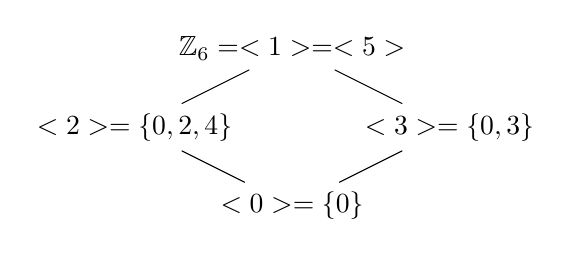
\begin{tikzpicture}
        \node (a1) at (0,2) {$\mathbb{Z}_6=<1>=<5>$};
        \node (a2) at (-2,1) {$<2>=\{0,2,4\}$};
        \node (a3) at (2,1) {$<3>=\{0,3\}$};
        \node (a4) at (0,0) {$<0> = \{0\}$};

        \draw[-] (a1) -- (a2);
        \draw[-] (a1) -- (a3);
        \draw[-] (a4) -- (a2);
        \draw[-] (a4) -- (a3);
    \end{tikzpicture}
\end{center}

\textcolor{blue}{Example 2.5.2:} Consider $\mathbb{Z}_8 = \{0,1,2,3,4,5,6,7\}$. Then we have
\begin{center}
    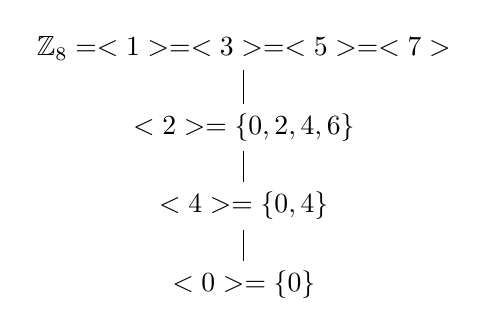
\begin{tikzpicture}
        \node (a1) at (0,3) {$\mathbb{Z}_8 = <1> = <3> = <5> = <7>$};
        \node (a2) at (0,2) {$<2> = \{0,2,4,6\}$};
        \node (a3) at (0,1) {$<4> = \{0,4\}$};
        \node (a4) at (0,0) {$<0> = \{0\}$};

        \draw[-] (a1) -- (a2);
        \draw[-] (a2) -- (a3);
        \draw[-] (a3) -- (a4);
    \end{tikzpicture}
\end{center}

\textcolor{blue}{Example 2.5.3:} Consider $S_3 = \{(1), (1 \ 2), (1 \ 3), (2 \ 3), (1 \ 2 \ 3), (1 \ 3 \ 2)\}$. Then we have
    \begin{center}
        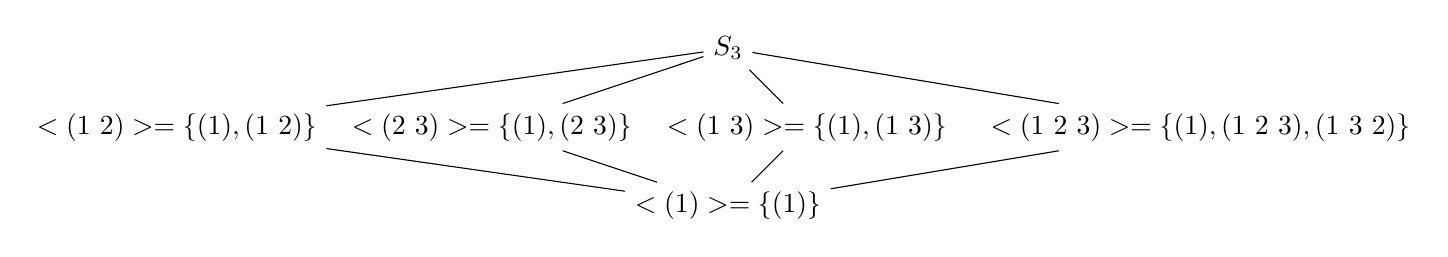
\begin{tikzpicture}
            \node (a1) at (0,2) {$S_3$};
            \node (a2) at (-7,1) {$<(1 \ 2)> = \{(1), (1 \ 2)\}$};
            \node (a3) at (-3, 1) {$<(2 \ 3)> = \{(1), (2 \ 3)\}$};
            \node (a4) at (1, 1) {$<(1 \ 3)> = \{(1), (1 \ 3)\}$};
            \node (a5) at (6, 1) {$<(1 \ 2 \ 3)> = \{(1), (1 \ 2 \ 3), (1 \ 3 \ 2)\}$};
            \node (a6) at (0,0) {$<(1)> = \{(1)\}$};

            \draw[-] (a1) -- (a2);
            \draw[-] (a1) -- (a3);
            \draw[-] (a1) -- (a4);
            \draw[-] (a1) -- (a5);
            \draw[-] (a6) -- (a2);
            \draw[-] (a6) -- (a3);
            \draw[-] (a6) -- (a4);
            \draw[-] (a6) -- (a5);
        \end{tikzpicture}
    \end{center}

\newpage
\section{Chapter 3: Quotient Groups and Homomorphisms}
\subsection{Definitions and Examples}

\textcolor{purple}{Definition 3.1.1:} Let $\phi:G \longrightarrow$ be a group homomorphism. The \textcolor{purple}{kernel} of this map is $\ker{(\phi)} = \{g \in G: \phi(g) = e_H\}$.

\textcolor{red}{Proposition 3.1.1:} Let $\phi:G \longrightarrow H$ be a group homomorphism. Then
\begin{enumerate}
    \item $\phi(e_G) = e_H$
    \item $\phi(g^{-1} = \phi(g)^{-1})$
    \item $\phi(g^n) = \phi(g)^n$
    \item $\ker{(\phi)} \leq G$
    \item $\Im{(\phi)} \leq H$ where $\Im{(\phi)} = \{h \in H: \phi(g) = h \text{ for some } g \in G\}$.
\end{enumerate}

Let us sketch a proof for the first statement in the proposition above.

\textbf{Proof:} We have
\begin{align*}
    e_G \cdot e_G = e_G &\Longrightarrow \phi(e_G) = \phi(e_G \cdot e_G) \\
    &\Longrightarrow \phi(e_G) = \phi(e_G) \cdot \phi(e_G).
\end{align*}
Since $\phi(e_G) \in H$ and $\phi(e_G) - \phi(e_G) \cdot \phi(e_G)$, we must have that $\phi(E_G) = e_H$. $\square$

\textcolor{purple}{Definition 3.1.2:} For $N \leq G$ and $g \in G$, $gN = \{gn: n \in N\}$ is a \textcolor{purple}{left coset} of $N$ in $G$ and $Ng = \{ng: n \in N\}$ is a \textcolor{purple}{right coset} of $N$ in $G$. An element $x \in gN$ or $x \in Ng$ is called a \textcolor{purple}{coset representative}.

Now, let $G$ be a group with $N \leq G$. Given any two left cosets of $N$ in $G$, say $g_1N$ and $g_2N$, we can combine the cosets by defining $g_1N \cdot g_2N = (g_1g_2)N$, where $\cdot$ is the rule that we are defining and $(g_1g_2)$ is the product of $g_1$ and $g_2$ in $G$. In general, this rule is \textit{not} an operation.

\textcolor{purple}{Definition 3.1.3:} $N \leq G$ is a normal subgroup if $gN = Ng$ $\forall g \in G$. Equivalently, $gNg^{-1} = N$ $\forall g \in G$. Notationally, we say $N$ is a normal subgroup of $G$ by saying $N \vartriangleleft G$. In terms of $N_G(N)$ (the normalizer of $N$ in $G$), $N$ is normal in $G$ if and only if $N_G(N) = G$.

\textcolor{red}{Theorem 3.1.1:} Let $G$ be a group with $N \leq G$. Then the following are equivalent:
\begin{enumerate}
    \item $N \trianglelefteq G \Longleftrightarrow gNg^{-1} = N \ \forall g \in G$
    \item $N_g(N) = G$
    \item $gN=Ng \ \forall g G$
    \item $g_1N \star g_2N := (g_1g_2)N$ utilizes a well-defined operation on the set of left cosets of $N$ in $G$
    \item $gNg^{-1} \subseteq N \ \forall g \in G$
\end{enumerate}

We will utilize a chain of proofs for the theorem above. First, we prove that the first item implies the second.
\textbf{Proof ($1 \Longrightarrow 2$):} Let $G$ be a group with $N \leq G$. Assume $N \trianglelefteq G$. Then, by definition, $gNg^{-1} = N \ \forall g \in G$. Therefore, $g \in G \Longrightarrow g \in N_G(N)$, so $N_G(N) = G$. $\square$

\textbf{Proof ($2 \Longrightarrow 3$):} Assume $N_G(N) = G$. First, we claim that $gN \subseteq Ng$. Let $gn \in gN$. Since $g \in N_G(N), \ gng^{-1} \in N$. Then $gng^{-1} = n_2 \in N$. We have $gng^{-1} = n_2 \Longrightarrow gn = n2g \in Ng$, then $gN \subseteq Ng$.\\
Next, we claim that $Ng \subseteq gN$. In doing so, we claim $g^{-1} \in N_G(N)$. We have
\begin{align*}
    g^{-1} \in N_G(N) &\Longrightarrow g^{-1} \in G: g^{-1}N(g^{-1})^{-1} = N \\
    &\Longrightarrow g^{-1}n_1 = n_2g^{-1} \\
    &\Longrightarrow gg^{-1}n_1 = gn_2g^{-1} \\
    &\Longrightarrow n_1 = gn_2g^{-1} \\
    &\Longrightarrow n_1g = gn_2g^{-1}g \\
    &\Longrightarrow n_1g = gn_2  
\end{align*}
Now, note that $n_1g \in Ng$ and $gn_2 \in gN$, so $n_1g = gn_2 \Longrightarrow n_1g \in gN \Longrightarrow Ng \subseteq gN$. $\square$

\textbf{Proof ($2 \Longrightarrow 3$):} Assume $gN = Ng \ \forall g \in G$. Suppose $g_1N = g_2N$ and $h_1N = h_2N$. We need to show $(g_1h_1)N = N(g_2h_2)$. Note that 
\begin{align*}
    g_1N = g_2N &\Longrightarrow \exists n_1 \in N : g_2^{-1}g_1=n_1 \text{ and }\\
    h_1N = h_2N &\Longrightarrow \exists n_2 \in N : h_2^{-1}h_1=n_2.
\end{align*}
Solving for $g_1$ and $h_1$ gives us $g_1 = g_2n_1$ and $h_1=h_2n_2$. Then we have
\begin{align*}
    (g_1h_1)N &= (g_2n_1h_2n_2)N \\
    &= g_2n_1h_2n_2N \\ 
    &= g_2n_1h_2N \\
    &= g_2h_2n_3N \\
    &= g_2h_2N \\
    &=(g_2h_2)N 
\end{align*}

\end{document}